%%%%%%%%%%%%%%%%%%%%%%%%%%%%%%%%%%%%%%%%%%%%%%%%%%%%%%%%%%%%%%
% ECE 445 SENIOR DESIGN TEMPLATE
%%%%%%%%%%%%%%%%%%%%%%%%%%%%%%%%%%%%%%%%%%%%%%%%%%%%%%%%%%%%%
\documentclass[letterpaper,10pt]{article}

%%%%%%%%%%%%%%%%%%%%%%%%%%%%%%%%%%%%%%%%%%%%%%%%%%%%%%%%%%%%%
% The preamble starts here.
% You can add other packages that you want to use by using
% \usepackage command in the preamble.
% However, DO NOT change the settings that are already placed
% below unless you really know what you are doing.
%%%%%%%%%%%%%%%%%%%%%%%%%%%%%%%%%%%%%%%%%%%%%%%%%%%%%%%%%%%%%

% some commonly used packages
\usepackage{siunitx}
\usepackage{graphicx}
\usepackage{color,soul}
\usepackage{amsmath}
\usepackage{amsthm}
\usepackage{amsfonts}
\usepackage{setspace}
\usepackage{longtable}
\usepackage{url}
\usepackage{pdfpages}
\usepackage{float}
\usepackage{rotating}
\usepackage{caption}
\usepackage{booktabs}  % professional-looking tables
\usepackage{multicol} %used for getting multicolumn without page-break
\usepackage{multirow}	% multi-row tables
\usepackage{array}		% define column format of a table
\usepackage[colorlinks=true,linkcolor=black,citecolor=black]{hyperref}
\usepackage[top=1.1in, bottom=1.1in, left=1.1in, right=1.1in]{geometry}% set the page margins to 1 inch

% use the fancyhdr package to maintain the format of the page numbers,
% which is useful when the text color is changed
\usepackage{fancyhdr}
\fancyhf{}
\renewcommand{\headrulewidth}{1pt}
\renewcommand{\footrulewidth}{0pt}
\fancyfoot[C]{\textcolor{black}{\thepage}}
\fancyhead[L]{
\includegraphics[width=2cm]{University-of-Illinois-logo.jpg}}
\fancyhead[R]{\small{Infantry I.F.F. Final Report - Meyers \& Prince}}

% paralist provides extended list environments
\usepackage{paralist}
\setlength{\plitemsep}{0pt}

% define the color for section and subsection titles
\usepackage{xcolor}
\definecolor{titlecolor}{RGB}{31,73,125}
\definecolor{subtitlecolor}{RGB}{79,129,189}

% change the style of the section and subsection titles
\usepackage{titlesec}
\titleformat{\section}{\color{titlecolor}\Large\bf}{\color{titlecolor}\thesection}{0.8em}{}
\titleformat{\subsection}{\color{subtitlecolor}\large\bf}{\color{subtitlecolor}\thesubsection}{1em}{}
\titleformat{\subsubsection}{\color{subtitlecolor}\normalsize\bf}{\color{subtitlecolor}\thesubsubsection}{1.2em}{}
\titlespacing{\section}{0pt}{0em}{0em}
\titlespacing{\subsection}{6pt}{0em}{0em}
\titlespacing{\subsubsection}{12pt}{0em}{0em}



% change the style of the table of contents
\usepackage{titletoc}
\titlecontents{section}[1.5em]{}{\contentslabel{1.5em}}{\hspace*{-1.5em}}{\titlerule*[0.5pc]{.}\contentspage}
\titlecontents{subsection}[3em]{}{\contentslabel{2.1em}}{\hspace*{-2.1em}}{\titlerule*[0.5pc]{.}\contentspage}
\titlecontents{subsubsection}[5.1em]{}{\contentslabel{2.7em}}{\hspace*{-2.7em}}{\titlerule*[0.5pc]{.}\contentspage}

% command for centering texts in a fixed width table cell
\newcommand{\centpcol}{\leftskip\fill \rightskip\fill}

% command for setting the style of the appendix titles
\newcommand{\setappenstyle}{
	\titleformat{\section}{\color{titlecolor}\Large\bf}{\color{titlecolor}Appendix \Alph{section}}{0.8em}{}
	\titlecontents{section}[0em]{}{Appendix \thecontentslabel \hspace{1em}}{}{\titlerule*[0.5pc]{.}\contentspage}
}

\makeatletter
\newcommand{\skipitems}[1]{%
	\addtocounter{\@enumctr}{#1}%
}

% define the style of the title of the paper
\newcommand{\thetitle}[1]{\title{\begin{huge}{\bf #1}\end{huge} \color{subtitlecolor}\rule[25pt]{\textwidth}{1pt}}}

% define the style of the author
\newcommand{\theauthor}[3]{
	\author{\vspace{.4in}\\
	\textcolor{black}{By}\\
	#1
	\vspace{1in}\\
	\textcolor{black}{ECE 445 Final Report -} #2\\
	\textcolor{black}{TA:} #3
	\vspace{1in}}
}

% define the style of figure's caption
\newcommand{\figcap}[1]{
	\captionsetup{format=plain,font={small,color=subtitlecolor,singlespacing},margin={0pt,0pt}}
	\caption{\textcolor{subtitlecolor}{#1}}
	\vspace{-5pt}
}

% define the style of table's caption
\newcommand{\tablecap}[1]{
	\captionsetup{format=plain,font={bf,normalsize,singlespacing,color=black},margin={0pt,0pt}}
	\caption{\textcolor{black}{#1}}
	\vspace{-5pt}
}


\newcommand{\buildtoc}{
	\clearpage
	\singlespacing
	\tableofcontents
	\onehalfspacing
}

% set indentations and the space between paragraghs
\setlength{\parindent}{0pt}
\setlength{\parskip}{8pt}

\setcounter{secnumdepth}{4}

\titleformat{\paragraph}
{\normalfont\small\bfseries\color{subtitlecolor}}{\theparagraph}{1em}{}
\titlespacing*{\paragraph}
{18pt}{3.25ex plus 1ex minus .2ex}{1.5ex plus .2ex}

%%%%%%%%%%%%%%%%%%%%%%%%%%%%%%%%%%%%%%%%%%%%%%%%%%%%%%%%%%%%%
% PREAMBLE ENDS HERE, DOCUMENT STARTS BELOW
%%%%%%%%%%%%%%%%%%%%%%%%%%%%%%%%%%%%%%%%%%%%%%%%%%%%%%%%%%%%%

\begin{document}

% don't change these
\pagestyle{empty}
\doublespacing

% put the title of your project here. DO NOT include the brackets.
\thetitle{{I.F.F. (Identification Friend or Foe) System}}

% put your names here. seperate by \\. DO NOT include the brackets.
\theauthor{
	{Eric Meyers (emeyer7)}\\
	{Noah Prince (nprince2)}\\
}
{ % put the semester info here. DO NOT include the brackets.
	{Spring 2016}
}
{ % put your TA's name here. DO NOT include the brackets.
	{Braedon Salz}
}

% put the date and project number here. DO NOT include the brackets.
\date{
{May 4th, 2016}\\
Project No. 11
\clearpage
}

% don't change these
\maketitle
\pagestyle{fancy}
\begin{spacing}{1.15}


% build the table of contents. 
\color{black}
\buildtoc
\pagenumbering{gobble}
\clearpage
\setcounter{page}{1}
\pagenumbering{arabic}

%SECTION - Introduction
\section{Introduction}
Briefly review and update the material from your proposal, presentation, and individual reports. Describe the function, and show the block diagram (which will most likely be your Figure 1 or Figure 1.1), being sure to cite the figure directly in the text (see Section 5.2). Describe briefly the blocks into
which the project has been divided. Give the performance requirements as they appear in the final version of your proposal. Describe any block‐level changes made to the design during the semester. Show that you understand the key factors in the performance of your project. Be quantitative if
possible. If in doubt, seek advice.

\subsection{System Block Diagram}
\begin{figure} [H]
	\centering
	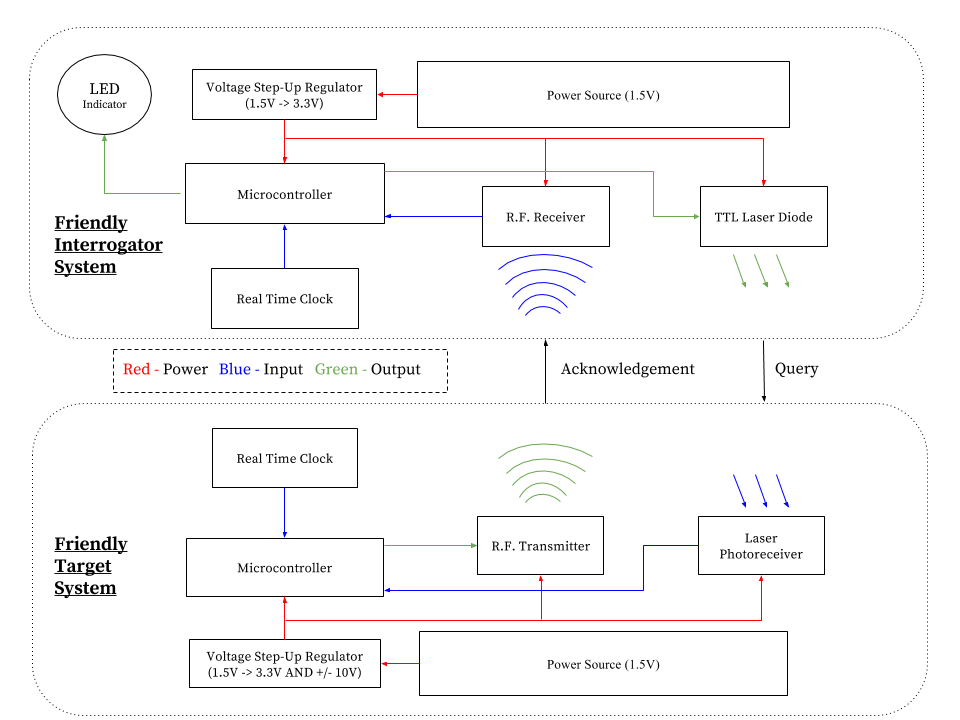
\includegraphics[scale=0.45]{System_Block_Diagram.png}
	\caption{System Block Diagram\label{fig:system-block-diagram}}
\end{figure}

\subsection{System Level Requirements}


%SECTION - Design
\section{Design}


%DESIGN - FRIENDLY INTERROGATOR UNIT
\subsubsection{Design Procedure} 
Discuss your design decisions for each block at the most general level: What alternative approaches tothe design are possible, which was chosen, and why is it desirable? Introduce the major design equations or other design tools used; show the general form of the circuits and describe their functions.

%DESIGN - FRIENDLY TARGET UNIT
\subsubsection{Design Details}
Present the detailed design, with diagrams and component values. Show how the design equations were applied. Give equations and diagrams with specific design values and data. Place large data tables in an appendix.  Circuit diagrams that are too large to be readable on a single page should be broken into pieces for presentation.  The full diagram may be included in an appendix.  Use photographs only as necessary and treat them, along with all other graphics except tables, as figures.

\section{Verification}
Discuss the Requirement and Verification Table from your design review. Including the table in an appendix will help avoid lengthy and tedious narrative description in the main text, which may not be of immediate interest to your imagined audience of managers. Do not discuss low‐level requirements unless they failed to verify, or you found that they were critical in some unexpected way, or you need to makes changes—for instance, to the tolerances or acceptable ranges of quantitative results. It is important to hit the main points and explain any requirement that is not verified, but keep the discussion concise and refer interested readers to the appendix for details. Note that the design procedure, design details, and design verification can be organized in different ways. The Word template provided by the ECE 445 staff puts the first two in one chapter and the second in another; however, a separate chapter for each is also common, with chapter sections reiterating the main project components. If you do the latter, avoid unnecessary repetition of component descriptions. Another option, though rarely used, is to organize the report according to components or blocks, with each chapter describing the design procedure, details, and verification for a single component or block.

\section{Costs}
Labor cost estimates should use the following formula for each partner:
ideal salary (hourly rate)  actual hours spent  2.5 include estimates for electronics and machine shop hours, as applicable. For parts, use real values when you know them; make realistic estimates otherwise. List both the retail cost and what you or the department paid (in this case you may list lab‐owned pieces as free).  If the project might be commercially viable, estimate the cost of mass‐production by listing bulk‐purchase costs. Make sure any tables are numbered appropriately, given titles, and cited directly in the text.  

\section{Conclusion}
Bring together, concisely, the conclusions to be drawn. It may be appropriate, depending on the nature of the project, to begin or end with a two‐ or three‐sentence executive summary. The reader needs to be convinced that the design will work. Summarize your accomplishments. If uncertainties remain, they should be pointed out, and alternatives, such as modifying performance specifications, should be spelled out to deal with foreseeable outcomes. Use  words, not equations or diagrams. Devote a section to ethical considerations with reference to the IEEE Code of Ethics and any other applicable code (e.g., the AMA Code of Medical Ethics for certain bioengineering projects).

\section{References}
Follow the IEEE reference styles provided in this document for various kinds of sources. If you need to
cite something for which there is no example, simply use common sense and provide—in a neat and
orderly manner emulating the IEEE reference style—the information necessary for another researcher
to find that source.  
References [1]–[3] are examples of a manual, datasheet, and web page, respectively. References [4]–[7]
are more standard, scholarly sources: a book, chapter in an edited book, journal article, and conference
proceedings. Reference [8] is a technical report, and reference [9] is class notes. Cite all references
consecutively in the text, as is done here. (ECE Editorial Services provides a more detailed description of
IEEE reference style on its wiki: http://go.illinois.edu/ecethesis .)


%SECTION - References
\clearpage
\bibliographystyle{IEEE_ECE}
% include the BibTex file here to build reference
\bibliography{Citations}\addcontentsline{toc}{section}{Reference}
\clearpage
\section*{Appendix}

\end{spacing}
\end{document}

